%% The following is a directive for TeXShop to indicate the main file
%%!TEX root = diss.tex

\chapter{Cross-modal word identification}
\label{chap:sent}

%This chapter investigates perceptual learning with a different bias than lexical, by using sentential context to bias participants towards a particular word.

\section{Motivation}

The largest perceptual learning effect in this dissertation was found in Experiment 1 in the No Attention/ Word-medial condition, which is the condition that was the least likely to promote a perception-oriented attentional set in listeners.
The lexical decision task is a comprehension-oriented task, so the comprehension-oriented attentional set is the default attentional set.
Participants with no manipulation promoting a perception-oriented attentional set would have maintained this default attentional set.
The experiment in this chapter examines perceptual learning in larger sentence contexts, as opposed to lexically guided perceptual learning in single word paradigms.
Using sentences ending with final target words that contain a modified /s/ category, semantic predictability is used in conjunction with lexical bias to boost linguistic expectations.
The linguistic expectation exploited in Chapter~\ref{chap:lexdec} was a lexical expectation.
Hearing part of a word increases a listener's expectation for hearing the rest of that word.
But as the words are presented in isolation in the lexical decision task, all words have equal likelihood of occurring.
No particular expectations are present prior to hearing the initial sounds of the word.
In a sentence context, however, expectations of a particular word can be boosted by the words preceding it.
If the expectation for a word is increased, the expectations for the sounds within it would be increased as well.


For our purposes, semantic predictability refers to how predictable the final word in a sentence is \citep{Kalikow1977}.
Example (1) is a high predictability sentence and Example (2) is an unpredictable sentence.
Although the final word is the same in both, the preceding sentence cues the final word in the predictable sentence, but not in the unpredictable one.
Semantic predictability does not reference formal models of semantics explicitly, but is rather more about world knowledge.

\ex[exno=1]
The cow gave birth to the calf.
\xe
\ex[exno=2,aboveexskip=0pt]
She is glad Jane called about the calf.
\xe


In general, high predictability sentences contain less signal information, but are easier to process and understand.
For example, semantic predictability in production studies is associated with phonetic reduction (particularly duration of words and sounds) independent of lexical factors like frequency and neighborhood density \citep{Scarborough2010, Clopper2008}.  
In speech perception work, semantic predictability and lexical bias have been found to have similar effects on phoneme categorization \citep{Connine1987,Borsky1998}.
Sentences with higher semantic predictability are more intelligible in noise, particularly for native speakers \citep[and others]{Kalikow1977, Mayo1997, Fallon2002, Bradlow2007}.
Similarly, in phoneme restoration tasks, semantic predictability increases the bias for a listener to hear a complete word, which may account for the increased intelligibility.
However, this increased bias is coupled with an increased sensitivity in detecting missing sounds for semantically predictable words \citep{Samuel1981}.

\citet{Samuel1981} proposes that high predictability sentences place a lower cognitive load on the perceptual system.  
The lower cognitive load allows for more cognitive resources to be allocated to the primary perception-oriented task, resulting in greater perceptual sensitivity.
\citet{Mattys2011} manipulated cognitive load through easier or harder concurrent visual search tasks during a phoneme categorization task.
Mirroring the phoneme restoration results, Mattys and colleagues found greater perceptual sensitivity in conditions with lower cognitive load.
In both of these cases, the goal of the listener was oriented towards perception.
A lower cognitive load on the perceptual system may allow more cognitive resources (including attention) to be allocated to perception.
In a comprehension-oriented task, lower cognitive load would not necessarily always result in greater perceptual sensitivity. 
If a listener's end goal is not perception of a specific production of a speech sound, then performance on the task would not necessarily be increased by attending further to perception.

There are many possible outcomes for perceptual learning in this experiment.
Many theoretical frameworks do not make explicit predictions about how the perceptual system will be updated in the context of full sentences.
Most models of speech perception end at perception of words.
In a sentence like Example (1), perceiving individual words is likely not the goal.
For instance, independently perceiving the word \emph{to} does not aid in comprehending the meaning of the sentence.
Instead, comprehension is likely more oriented towards the relations between concepts and perceiving phrases or multiword chunks.
If the perceived chunk is larger than a word, are the fine details still as faithfully encoded as they are for words in isolation?
Even if the fine details are encoded, are they reliable enough evidence for perceptual learning?
The experiment reported here takes a first pass at answering some of these questions, and sets the stage for future inquiry into perceptual learning from sentences. 

One promising avenue for exploring this chapter's research questions lies in the reliability of evidence, which has been shown previously to be crucial for perceptual learning \citep{Kraljic2008, Kraljic2008a}.
If ambiguous productions are accompanied by a video of the speaker holding a pen in their mouth, then no perceptual learning is observed \citep{Kraljic2008}.
Likewise, if listeners are first exposed to typical tokens, and then exposed to atypical tokens, no perceptual learning is observed.
If the order is flipped (atypical tokens first), then perceptual learning effects are present \citep{Kraljic2008}.
If there is a linguistic context that conditions a greater variability, then modified tokens in those contexts will not cause perceptual learning \citep{Kraljic2008a}.
However, the unlearned modification must lie within the range of variability conditioned by the context.
For /s/ in /st\textturnr/ clusters, where /s/ becomes more /\textesh/ like due to coarticulation, a more /\textesh/-like modification will not be learned.
Presumably, modifications that lay outside of the variability conditioned by the context will still be learned.
Kraljic and colleagues argue from these studies that listeners will attribute variation to the context as much as possible, and only fall back to updating perceptual categories when no other explanation is available.

Extended beyond single words, reliability can be thought of in terms of perceived carefulness of a word production.
In an experimental setting, every stimulus is carefully curated by the experimenter.
However, both in the laboratory and outside, words in isolation are produced longer and more clearly than their counterparts in full sentences.
Words in isolated sentences are going to be produced less clearly than words in isolation (though not necessarily unintelligibly).
Words in spontaneous conversation are likely to be the least clear, as seen in the ``massive reduction'' in the Buckeye corpus \citep{Johnson2004, Dilts2013}.
All of these factors are dependent on aspects of the sentence (focus, clause type, etc.) or of the speech style, so words in casual conversation will be less clear than words in a formal presentation.

From a perception standpoint, the more clear an acoustic token, the more signal information is available to be processed.
Clear tokens typically have longer durations, increased intensity, and more distinct formants \citep{Krause2004}.
A listener would view tokens that were produced more clearly or with greater care as more reliable productions for that speaker.
Listeners have been found to recognize careful and casual speech equally well, but signal information is used more in careful speech \citep{Sumner2015}.
If we extend the argument by Kraljic and colleagues, it would predict that sentences should have less perceptual learning than words in isolation because (some of) the variability of a word's production in a sentence can be attributed to the fact that the item is in a sentence context.
Additionally, given the propensity for acoustic reduction in high predictability contexts \citep{Scarborough2010}, words in predictable sentences would be even less reliable, leading to less perceptual learning.

This is not to say that sentences are ineffective in driving perceptual learning as compared to words in isolation.
From the literature on perceptual learning of foreign accents, sentences are extremely useful in learning to perceive nonnatively accented speakers \citep{Bradlow2008}.
For the purposes of learning an accent, sentences are probably better than words in isolation, as the greater context would allow for better identification of the words.
Differences in perceptual learning from native and nonnative speakers can also be seen in the contradictory findings of \citet{Sumner2011} and \citet{Kraljic2008}.
\citet{Sumner2011} found that listeners could update their perceptual categories constantly over the course of the experiment.
In contrast, \citet{Kraljic2008} found that listeners adapted to the first instances of the category that they heard and did not use subsequent tokens.
The nativeness of the exposure speaker differed in the two experiments.
Constant adaptation was found for a nonnative speaker \citep{Sumner2011} rather than a native speaker \citep{Kraljic2008}.
Listeners may be more biased toward typical native categories for native speakers, so that exposure to an initially typical category causes listeners to disregard the later atypical category as unreliable.
Listeners can therefore leverage their previous experience with native speakers more readily.
Listeners' previous experience does not as readily extend to nonnative speech, where interspeaker and intraspeaker variation is more prevalent, so constant adaptation and consistent token reliability would improve comprehension the most.

This dissertation largely adopts the predictive coding framework presented in \citet{Clark2013} to account for perceptual learning.
Reliability of sensory information is not directly addressed in Clark's exposition.
The basic form of his model, however, predicts that increasing expectations should always increase error signals.
In \citet[cited in \citet{Clark2013}]{Egner2010}, participants were exposed to faces and non-face objects (i.e., houses) embedded in white noise on a computer screen (static).
Participants who were told about the faces had equally-sized neuronal responses in the fusiform face area for face stimuli as for non-face stimuli.  
Participants who were not expecting to see faces showed neuronal responses in that area only for the face stimuli.
The mismatch between expectation and the perceived signal generated an error signal of similar magnitude to the signal itself.
If increased expectations result in increased error signals, perceptual learning should be largest for participants exposed to the modified category in higher predictability sentences.
If smaller perceptual learning effects are observed for those participants, then reliability weighting or attribution of error signals would be necessary in the model.

To test these predictions, a novel exposure paradigm was used in place of a lexical decision task.  
In this paradigm, participants are presented with sentences auditorily.  
Following the sentence, two pictures appear on the screen: one matching the final word of the sentence and the other a distractor. 
Participants are instructed to indicate which picture corresponds to the final word of the sentence.
Following exposure, participants completed the same categorization task as those in Experiments 1 and 2.
This experiment will validate lexical decision tasks for learning a single characteristic (/\textesh/-like /s/) in a context that is more closely resembling actual language use.
At the same time, this experiment provides a link between lexically-guided perceptual learning and experiments that use sentential stimuli for learning non-native accents \citep{Bradlow2008}.

\section{Methodology}

\subsection{Participants}

A total of 137 participants from the UBC population completed the experiment and were compensated with either \$10 CAD or course credit.  
The data from 39 nonnative speakers of English were excluded from the analyses.
No participants reported speech or hearing disorders.
This left data from 98 participants for analysis.
Twenty additional native English speakers participated in a pretest to determine sentence predictability, and 10 other native English speakers participated in a picture naming pretest.

\subsection{Materials}

One hundred and twenty sentences were used as exposure materials.  
The set of sentences consisted of 40 critical sentences, 20 control sentences and 60 filler sentences. 
The critical sentences ended in one of 20 of the critical words in Experiments 1 and 2 that had an /s/ in the onset of the final syllable.  
The 20 control sentences ended in the 20 control items used in Experiments 1 and 2, and the 60 filler sentences ended in the 60 filler words in Experiments 1 and 2.  
Half of all sentences were written to be predictive of the final word, and the other half were written to be unpredictive of the final word.  
Unlike previous studies using sentence or semantic predictability \citep{Kalikow1977}, unpredictive sentences were written with a range of sentence structures.
In all cases, the final words were plausible objects of lexical verbs and prepositions.
The high and low predictability filler sentences can be found in Tables~\ref{tbl:senthighfiller} and~\ref{tbl:sentlowfiller}, respectively.
The high and low predictability filler sentences with /\textesh/ words can be found in Tables~\ref{tbl:senthighsh} and~\ref{tbl:sentlowsh}, respectively.
Finally, the high and low predictability critical sentences can be found in Tables~\ref{tbl:senthighs} and~\ref{tbl:sentlows}, respectively.
Aside from the sibilants in the critical and control words, the sentences contained no sibilants (/s z \textesh\ \textyogh\ \textteshlig\  \textdyoghlig/).  
The same minimal pairs for phonetic categorization as in Experiments 1 and 2 were used.

\begin{table}[!ht]
\caption{High predictability filler sentences.}
\label{tbl:senthighfiller}
\small
\centering
\begin{tabular}{llc}
\toprule
Sentence                                                                     & Word        & Distractor  \\
\midrule
The oak tree grew from a tiny                                                & acorn       & pineapple   \\
The radio in the car didn't work with a bent                                 & antenna     & towel       \\
The clown made the girl an animal from a                                     & balloon     & pancake     \\
Everyday the panda had to eat a lot of                                       & bamboo      & boomerang   \\
The belt had an ornate                                                       & buckle      & hamburger   \\
The caterpillar came out of the cocoon a beautiful                           & butterfly   & crayon      \\
The hermit lived in a log                                                    & cabin       & parade      \\
They marked the date on the                                                  & calendar    & antler      \\
They rode to the pyramid on the back of a                                    & camel       & atom        \\
Right before the plane took off,  & & \\
the captain called the flight crew from the & cockpit     & doorknob    \\
The woman threaded the bowtie through her                                    & collar      & ladybug     \\
At the rodeo, the cattle were rounded up by the                              & cowboy      & ripple      \\
The baby rocked in her                                                       & cradle      & telephone   \\
The delivery man rang the                                                    & doorbell    & firewood    \\
He moved the wet laundry over to the                                         & dryer       & hydrant     \\
The tiny rodent terrified the big, grey                                      & elephant    & pepper      \\
The criminal wore a glove to not leave behind one                            & fingerprint & island      \\
The cook needed one more clove of                                            & garlic      & wheelbarrow \\
Red paint in hand, the youth tagged the building with                        & graffiti    & catapult    \\
The watery dinner had to be poured out with a                                & ladle       & lollipop    \\
The man reheated the leftover dinner in the                                  & microwave   & ukulele     \\
Every dinner plate came with a folded                                        & napkin      & toothpick   \\
The ballroom had a grand                                                     & piano       & dolphin     \\
The woman tied her hair back in a                                            & ponytail    & airport     \\
The adult frog developed from a                                              & tadpole     & bucket      \\
The acting company performed in an old                                       & theatre     & earmuff     \\
Her favorite burrito came wrapped in a flour                                & tortilla    & falafel     \\
The farm youth rode around on the                                            & tractor     & barbecue    \\
The train went under a mountain through a                                    & tunnel      & wagon       \\
The heavy rainfall could have been predicted by the                          & weatherman  & robot      \\
\bottomrule
\end{tabular}
\end{table}

\begin{table}[!ht]
\caption{Low predictability filler sentences.}
\label{tbl:sentlowfiller}
\small
\centering
\begin{tabular}{llc}
\toprule
Sentence                                                                     & Word        & Distractor  \\
\midrule
They clapped loudly for the                       & acrobat    & pillow      \\
The man liked to begin the day with an            & apple      & vampire     \\
Wearily, the woman built up her                   & campfire   & bagel       \\
He looked forward to freely available             & candy      & donkey      \\
The couple never agreed on the                    & cutlery    & butter      \\
He took pride in the renovated                    & darkroom   & candle      \\
They were enthralled by the                       & diamond    & kiwi        \\
While he lay on the ground, the boy played with a & feather    & broccoli    \\
To get any farther, they definitely needed a good & goalie     & waterfall   \\
He didn't know how to get to the                  & gondola    & honey       \\
They were a little frightened to board the        & helicopter & cannon      \\
The woman needed to borrow a                      & ladder     & flagpole    \\
He had to track down and get help from the        & librarian  & tornado     \\
They had a good view of the                       & lightning  & coffee      \\
Toward the end, they were running low on          & lumber     & anvil       \\
They liked how it looked on the                   & mannequin  & parrot      \\
On the way, they liked walking through the        & meadow     & cupcake     \\
The couple were looking forward to buying a       & minivan    & tugboat     \\
He finally made it to the                         & motel      & armadillo   \\
They went out for a quick bite to eat after the   & movie      & volleyball  \\
He really liked the look of the                   & mural      & monocle     \\
After a long night, he devoured the whole         & omelet     & hummingbird \\
On the field trip, they learned all about the     & painter    & pulley      \\
The boy cried when they took away the             & popcorn    & puppet      \\
The irate woman yelled at the                     & referee    & propeller   \\
When they were called, the group moved to the     & table      & helmet      \\
He didn't know about a problem with the           & teapot     & crowbar     \\
He had to remember to pick up the                 & tire       & parakeet    \\
Every day he dreaded the late afternoon           & traffic    & rowboat     \\
The woman kept a lookout for the                  & umbrella   & catamaran  \\
\bottomrule
\end{tabular}
\end{table}

Sentences were recorded by the same male Vancouver English speaker used in Experiments 1 and 2.  
Critical sentences were recorded in pairs, with one normal production and then a production of the same sentence with the /s/ in the final word replaced with an /\textesh/.  
The speaker was instructed to produce both sentences with comparable speech rate, speech style, and prosody.

\begin{table}[!ht]
\caption{High predictability sentences with /\textesh/ words.}
\label{tbl:senthighsh}
\small
\centering
\begin{tabular}{llc}
\toprule
Sentence                                                                     & Word        & Distractor  \\
\midrule
The bidding became frantic for the final item in the                     & auction     & accordion  \\
While waiting in line at the new bank,  & & \\
the woman read their introductory & brochure    & blueberry  \\
The woman only got a dime back after paying the                          & cashier     & laptop     \\
He could only kneel for a little while without a plump                   & cushion     & forklift   \\
Lava flowed down the volcano after the violent                           & eruption    & pumpkin    \\
The bear awoke from her winter                                           & hibernation & violin     \\
After jumping out of the plane, the woman opened her                     & parachute   & camera     \\
The doctor took the time to look in on every                             & patient     & crocodile  \\
While down with the flu, the woman invariably carried a clean            & tissue      & whirlpool  \\
The opera-goer found her row with the help of an                         & usher       & doormat   \\
\bottomrule
\end{tabular}
\end{table}

\begin{table}[!ht]
\caption{Low predictability sentences with /\textesh/ words.}
\label{tbl:sentlowsh}
\small
\centering
\begin{tabular}{llc}
\toprule
Sentence                                                                     & Word        & Distractor  \\
\midrule
The woman couldn't wait to fill up the        & bookshelf  & muffin     \\
The whole family travelled for an hour to the & coronation & waffle     \\
He did not look forward to the                & handshake  & raccoon    \\
He gave a wide berth to the                   & machine    & kitten     \\
They dragged their feet on the way to the     & mansion    & treadmill  \\
He had a hard time with                       & meditation & beekeeper  \\
They were deeply worried about the            & militia    & peanut     \\
He went on and on about the                   & milkshake  & elbow      \\
For winter break, he wanted to go to the      & ocean      & iguana     \\
He could finally get a new                    & windshield & koala     \\
\bottomrule
\end{tabular}
\end{table}

\begin{table}[!ht]
\caption{High predictability sentences with target /s/ words.}
\label{tbl:senthighs}
\small
\centering
\begin{tabular}{llc}
\toprule
Sentence                                                                     & Word        & Distractor  \\
\midrule
At the carnival the girl rode a unicorn around the & carousel & pirate \\
A deep moat protected the old & castle & martini \\
The encore from the pop duo perfected the whole & concert & earplug \\
From the bakery he got a flaky, buttery & croissant & windmill \\
After her world trip, & & \\
the traveller had a little money leftover in every local & currency & elevator \\
When the computer locked up, he couldn't move the & cursor & clover \\
The lady returned the bow with a formal & curtsy & gavel \\
The critic raved about the ballet and the lead & dancer & cricket \\
Long ago, a comet hit the earth, killing every big & dinosaur & bandana \\
Water poured into the bath tub from the & faucet & doughtnut \\
After millennia, the bone in the riverbed turned into a & fossil & menorah \\
The name 'Milky Way' can perfectly depict our & galaxy & kayak \\
We no longer worry about the plague due to modern & medicine & cucumber \\
In the heated aerial battle, neither pilot could lock on with a & missile & cookie \\
Rain fell every day in India during the & monsoon & gargoyle \\
The man wrote on the paper with a graphite & pencil & trombone \\
The woman got an over-the-counter drug at her local & pharmacy & kettle \\
From the cap of the new grad hung a golden & tassel & guitar \\
The New Yorker flagged down a & taxi & ribbon \\
The traffic cop alerted the driver by blowing her & whistle & ravioli \\
\bottomrule
\end{tabular}
\end{table}

\begin{table}[!ht]
\caption{Low predictability sentences with target /s/ words.}
\label{tbl:sentlows}
\small
\centering
\begin{tabular}{llc}
\toprule
Sentence                                                                     & Word        & Distractor  \\
\midrule
They got back in line for the & carousel & pirate \\
He dreaded the long walk to the & castle & martini \\
He prepared night and day for the & concert & earplug \\
The man had a craving for a & croissant & windmill \\
They weren't worried about the different & currency & elevator \\
The man could never find the & cursor & clover \\
The girl didn't want to make a & curtsy & gavel \\
The boy wanted to become a better & dancer & cricket \\
The boy really wanted to ride the & dinosaur & bandana \\
The woman hoped to get a working & faucet & doughtnut \\
No one knew where to find the & fossil & menorah \\
The man talked at length about the & galaxy & kayak \\
With that GPA, they could have a career in & medicine & cucumber \\
The boy wanted to build a toy & missile & cookie \\
On their picnic, they avoided the & monsoon & gargoyle \\
The woman looked frantically for her & pencil & trombone \\
The woman loved her work at the & pharmacy & kettle \\
He worried about the color of the & tassel & guitar \\
The woman had no luck getting a & taxi & ribbon \\
The boy ran away when he heard the & whistle & ravioli \\
\bottomrule
\end{tabular}
\end{table}

As in Experiments 1 and 2, the critical items were morphed together into an 11-step continuum using STRAIGHT \citep{Kawahara2008}; only the final word in each sentence was morphed. 
The preceding words were the synthesized versions of the sentence with the correct /s/ production to minimize artifacts of the morphing algorithm.  
The control and filler items were also processed and resynthesized to ensure consistent quality.  
The ambiguous point selection was based on the pretest performed for Experiment 1 and 2 exposure items.  
The ambiguous steps of the continua chosen corresponded to the 50\% cross over point in Experiment 1.

Acoustic distances between exposure tokens, categorization tokens, and their original productions were multidimensionally scaled.  In Figure~\ref{fig:exp3mds}, the original productions are separated again by the first dimension, which corresponds to the centroid frequency of the sibilant.
The categorization tokens are predictably in between the original productions and offset in the second dimension due to their different position in the word.
The exposure tokens for Experiment 3 fit in between the original productions and the categorization tokens.

\begin{figure*}[ht]
\caption{Multidimensional scaling of the acoustic distances between the sibilants of original productions, categorization tokens and the exposure tokens in Experiment 3. Note that the only Isolation tokens are the Categorization tokens.}
\label{fig:exp3mds}
\begin{center}
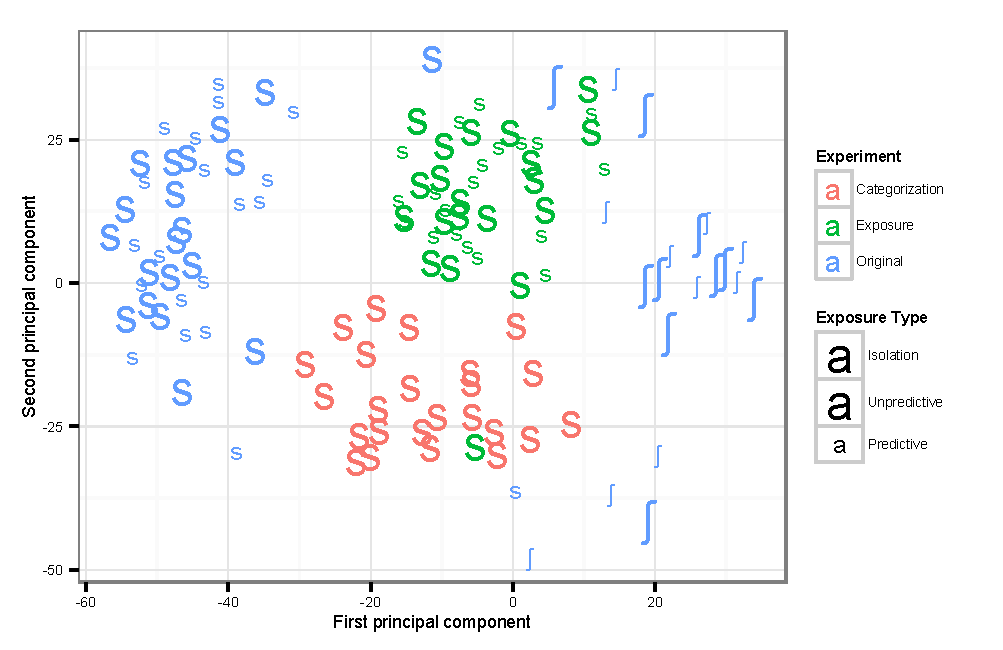
\includegraphics[width=\textwidth]{graphs/exp3_mds}
\end{center}
\end{figure*}

Sentences were pairs with two pictures apiece.
Pictures of 200 words, with 100 pictures for the final word of the sentences and 100 for distractors, were selected in two steps.  
First, a research assistant selected five images from a Google image search of the word, and then a single image representing that word was selected from amongst the five by me.  
To ensure consistent behavior in E-Prime \citep{PsychologySoftwareTools2012}, pictures were resized to fit within a 400x400 area with a resolution of 72x72 DPI and converted to bitmap format.  
Additionally, any transparent backgrounds in the pictures were converted to plain white backgrounds.

\subsection{Pretest}

The same twenty participants that completed the lexical decision continua pre-test also completed a sentence predictability task before the phonetic categorization task described in Experiment 1. 
Participants were compensated with \$10 CAD for both tasks, and were native North American English speakers with no reported speech, language or hearing disorders. 
In this task, participants were presented with the 120 exposure sentences with the final target word removed.
Participants were instructed to type in the word that came to mind when reading the fragment, and to enter any additional words that came to mind that would also complete the sentence.
There was no time limit for entry and participants were shown an example with the fragment ``The boat sailed across the...'' and the possible completions ``bay, ocean, lake, river''.  
Responses were collected in E-Prime \citep{PsychologySoftwareTools2012}, and were sanitized by removing miscellaneous keystrokes, spell checking, and standardizing variant spellings and plural forms.

From the sanitized data, responses were coded as either 0 if the target word was not present or 1 if it was.
For each sentence, the target response rate was calculated by averaging responses from all participants.
The target response rate was 0.49 (range 0-0.95) for predictive sentences and 0.03 (range 0-0.45) for unpredictive sentences.
Predictive sentences that had target response rates of 0.2 or less were rewritten.  
The predictive sentences for \emph{auction}, \emph{brochure}, \emph{carousel}, \emph{cashier}, \emph{cockpit}, \emph{concert}, \emph{cowboy}, \emph{currency}, \emph{cursor}, \emph{cushion}, \emph{dryer}, \emph{graffiti}, and \emph{missile} were rewritten to remove any syntactic or semantic ambiguities.
For instance, a common completion for the predictive sentence ``The youth tagged the wall with...'' was ``spray paint'' rather than ``graffiti''.
To promote the likelihood of ``graffiti'', the sentence was changed to ``Red paint in hand, the youth tagged the wall with...'', which would eliminate ``spray paint'' as a possible completion.

Five volunteers participated in another pretest to determine how suitable the pictures were at representing their associated word.  
All participants were native speakers of North American English, with reported corrected-to-normal vision. Participants were presented with a single image in the middle of the screen.  
Their task was to type the word that first came to mind, and any other words that described the picture equally well.  
There was no time limit and presentation of the pictures was self-paced. Responses were sanitized as above.  

Pictures were replaced if 20\% or less of the participants (1 of 5) responded with the target word and the responses were semantically unrelated to the target word. 
Five pictures were replaced, \emph{toothpick} and \emph{falafel} with clearer pictures and \emph{ukulele}, \emph{earmuff} and \emph{earplug} were replaced with \emph{rollerblader}, \emph{anchor} and \emph{bedroom}.  
All five replacements were for distractor words.

\subsection{Experiment design}

Participants were assigned to one of four groups from a 2x2 between-subject factorial design.
The first factor was whether the word containing the ambiguous sibilant was predictable from the preceding words or not  (Predictability: Predictive versus Unpredictive).
All participants were therefore exposed to a consistent 100 stimulus sentences with identical control and filler items for all participants.
The second factor was whether participants were given additional instructions about the sibilant or not (Attention: Attention versus No Attention).
Participants in the Attention condition received additional instructions that the speaker's ``s'' sounds were sometimes ambiguous, and to listen carefully to ensure correct responses.

\subsection{Procedure}

As in Experiments 1 and 2, participants completed an exposure task and a categorization task in E-Prime \citep{PsychologySoftwareTools2012}.  
For the exposure task, participants heard a sentence via headphones for each trial.  
Immediately following the auditory presentation, they were presented with two pictures on the screen.  
Their task was to select the picture on the screen that corresponded to the final word in the sentence they heard.  
The order was pseudorandom with the same constraints described in Experiment 1.
Half of the matching pictures were selected via one button and half via the other.

Each trial proceeded as follows.
A blank screen was presented for 250 ms.
Immediately following, a sentence was presented auditorily.
Following the auditory stimulus, two pictures and their respective buttons appeared on the screen.
For example, a sentence ending in ``dog'' would show a picture of a dog and ``1'' on one side of the screen, and a picture of a banana and ``5'' on the other side of the screen.
Participants had up to 3000 ms to respond which picture matched the final word in the sentence.
Feedback as to whether a response was detected was shown for 500 ms before the next trial began.
Participants were given a self-paced break after 50 trials.

Following the exposure task, participants completed the same categorization task described in Experiments 1 and 2.

Participants were given oral instructions explaining both tasks at the beginning of the experiment to remove experimenter interaction between exposure and categorization.
Written instructions were presented to participants at the beginning of each task as well.
The instructions for the exposure task given to participants assigned to an Attention condition included explicit reference to the modified sibilants.
Participants were told that ``this speaker's `s' sound is sometimes ambiguous'' and instructed to ``listen carefully so as to choose the correct response.''

\subsection{Analysis}

Response data and factors were transformed and analyzed in the same way as in Experiment 1 and 2.

\section{Results}

\subsection{Exposure}

Performance in the task was high, with accuracy near ceiling across all subjects (mean accuracy = 99.5\%, sd = 0.8\%).
Due to these ceiling effects, a logistic mixed-effects model of accuracy was not constructed.  
A linear mixed effects model for logarithmically-transformed reaction time was constructed with a similar structure as in Experiments 1 and 2.
Fixed effects were Trial (0-100), Trial Type (Filler, /s/, and /\textesh/), Attention (No Attention and Attention), Predictability (Unpredictive and Predictive), and their interactions.  
By-Subject and by-Word random effect structure was as maximal as permitted by the data, with by-Subject random slopes for Trial, Trial Type, Predictability, and their interactions and by-Word random slopes for Attention, Predictability, and their interaction. 
Trial Type was coded using treatment (dummy) coding, with Filler as the reference level. 
Deviance contrast coding was used for Predictability (Unpredictive = 0.5, Predictive = -0.5) and Attention (No attention = 0.5, Attention = -0.5).

\begin{figure*}[!ht]
\centering
\caption{Within-subject mean reaction time in the exposure phase of Experiment 3, separated out by Trial Type (Filler, /s/, and /\textesh/). Error bars represent 95\% confidence intervals.}
\label{fig:exp3exposert}
\begin{center}
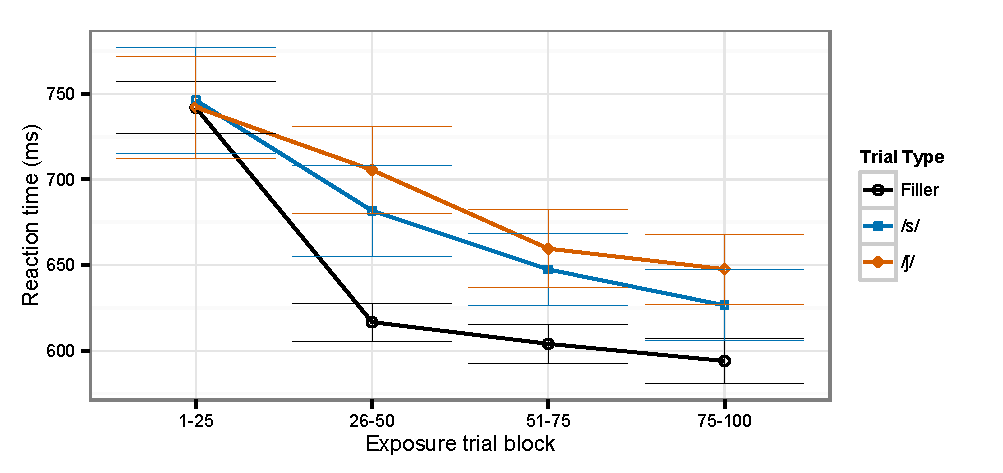
\includegraphics[width=0.95\textwidth]{graphs/exp3_exprt}
\end{center}
\end{figure*}

A significant effect was found for Trial ($\beta = -0.20, SE = 0.01, t = -11.0$), indicating that reaction time became faster over the course of the experiment.
There was a significant effect for Trial Type of /\textesh/ versus Filler ($\beta = 0.19, SE = 0.09, t = 2.1$), but not for /s/ versus Filler ($\beta = 0.11, SE = 0.09, t = 1.3$), suggesting that words with /\textesh/ in them were responded to more slowly than filler words or those with a modified /s/ in them.
There was a significant interaction between Trial and Trial Type of  /s/ versus Filler ($\beta = 0.05, SE = 0.02, t = 2.4$) and between Trial and Trial Type of /\textesh/ versus Filler ($\beta = 0.05, SE = 0.02, t = 2.9$), indicating that reaction time for words with /s/ or /\textesh/ in them did not become as fast across the experiment as those for filler words.
These results are shown in Figure~\ref{fig:exp3exposert}.
Note that the y-axis has a different scale than that used in Experiments 1 and 2 for reaction times.
Participants were faster in general in this task than in the lexical decision task.
Responses to predictable sentences (mean = 669 ms, SD = 321 ms) were not significantly faster than responses to unpredictable sentences (mean = 646 ms, SD = 299 ms), suggesting that performance was at floor.


\subsection{Categorization}

Responses with reaction times less than 200 ms or greater than 2500 ms were excluded from analyses. 
A logistic mixed effects model was constructed with Subject and Continua as random effects and continua Step as random slopes, with 0 coded as a /\textesh/ response and 1 as a /s/ response.  Fixed effects for the model were Step, Exposure Type, Attention, and their interactions, with deviance coding used for contrasts for Exposure Type (Unpredictive = 0.5, Predictive = -0.5) and Attention (No attention = 0.5, Attention = -0.5).


\begin{figure*}[!ht]
\caption{Proportion /s/ response along the 6 step continua as a function of Exposure Type and Attention in Experiment 3.  Error bars represent 95\% confidence intervals.}
\label{fig:exp3categ}
\begin{center}
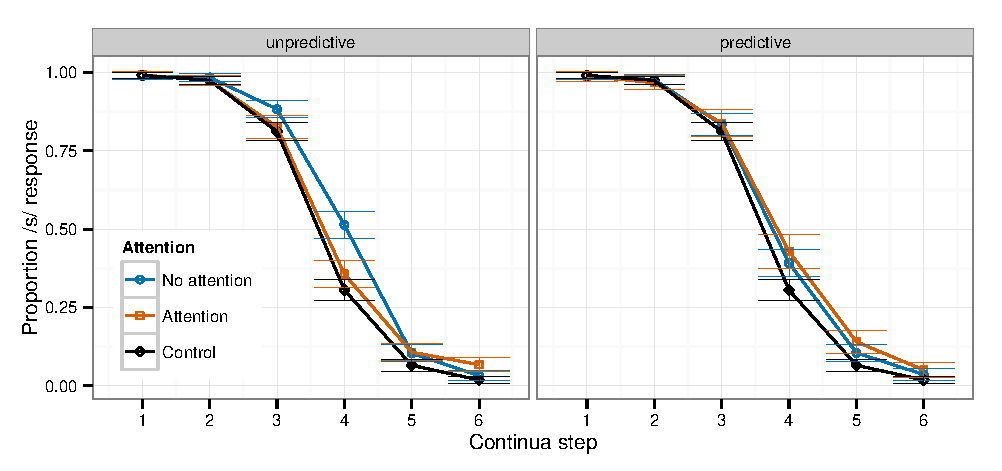
\includegraphics[width=\textwidth]{graphs/exp3_categresults}
\end{center}
\end{figure*}

As in the previous experiments, there was a significant effect of the intercept ($\beta = 0.52, SE = 0.20, z = 2.6, p < 0.01$) and of Step ($\beta = -2.49, SE = 0.19, z = -12.7, p < 0.01$).
Exposure Type ($\beta = 0.23, SE = 0.23, z = 0.97, p = 0.33$), Attention ($\beta = 0.30, SE = 0.21, z = 1.4, p = 0.15$), and their interaction ($\beta = 0.38, SE = 0.44, z = 0.9, p = 0.39$) are all not significant, despite the visible differences in Figure~\ref{fig:exp3categ}.
In Figure~\ref{fig:exp3categ}, there appears to be a similar interaction pattern as was seen for Experiment 1 (Figure~\ref{fig:exp1categ}).
Participants in the different attention conditions for Unpredictive exposure appear to differ in Step 4.
However, the lack of significance suggests that this may be less reliable or more localized to Step 4 than in Experiment 1.

\begin{figure*}[!ht]
\caption{Proportion /s/ response along the 6 step continua as a function of Exposure Type and Attention in Experiment 3 and the word-medial condition of Experiment 1.  Error bars represent 95\% confidence intervals.}
\label{fig:exp23categ}
\begin{center}
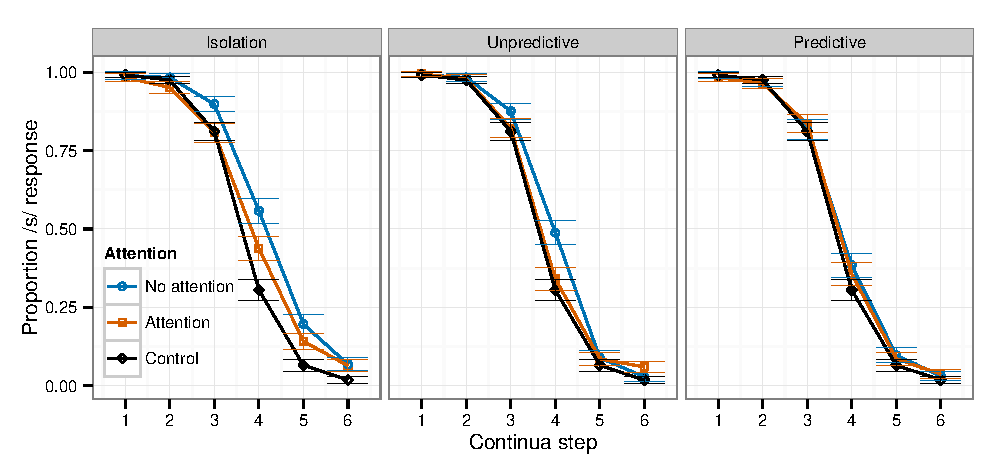
\includegraphics[width=\textwidth]{graphs/exp23_categresults}
\end{center}
\end{figure*}


As an additional comparison, the data from this experiment was combined with the subset of participants in Experiment 1 who were exposed to the same set of words (the word-medial condition).  
Exposure Type was recoded as a three-level factor, using treatment (dummy) contrast coding, with the Experiment 1 exposure (Isolation) as the reference level. 
An identically specified logistic mixed effects model was fit to this data set as to the initial data.  
In this model, there was a significant effect of Attention ($\beta = 0.74, SE = 0.32, z = 2.2, p = 0.02$), such that participants in Attention conditions were less likely to categorize the continua steps as /s/.  
Exposure Type had a marginal effect of Predictive compared to Isolation ($\beta = -0.43, SE = 0.23, z = -1.9, p = 0.05$), indicating that participants in the Predictive condition were less likely to categorize the continua as /s/ overall as compared to participants from Experiment 2. 
Step interacted with both Unpredictive as compared to Isolation ($\beta = -0.42, SE = 0.17, z = -2.4, p = 0.01$) and Predictive as compared to Isolation ($\beta = -0.32, SE = 0.14, z = -2.2, p = 0.02$).
These interactions indicate that the categorization functions for sentential stimuli had a steeper cross-over than the Isolation. 
As shown in Figure~\ref{fig:exp23categ}, the endpoints (Steps 5 and 6) for the sentential conditions are wholly overlapping with the control categorization for those steps.
While participants in the Unpredictive condition showed a shifted category boundary, the perceptual learning affected less of the continua than for participants in the Isolation condition.

An additional model was run with the reference level for Exposure Type as Predictive to check whether participants in the Predictive condition showed perceptual learning effects at all.
In the model with Predictive as reference, the intercept is no longer significant ($\beta = 0.44, SE = 0.28, z = 1.5, p = 0.12$), indicating perceptual learning was not robustly present in participants in the Predictive condition.  
The difference between the Predictive condition and the Isolation condition remains ($\beta = 0.77, SE = 0.32, z = 2.4, p = 0.01$), and, as above, the difference between Predictive and Unpredictive is not significant ($\beta = 0.42, SE = 0.31, z = 1.3, p = 0.17$).
These results indicate participants in the Predictive condition showed no perceptual learning effects, and participants in the Unpredictive condition were in between Predictive and Isolation, but not significantly different from either.  
Increasing the statistical power might separate the conditions further.


\section{Discussion}

The key finding of the current experiment is that modified categories embedded in words in meaningful sentences produce less perceptual learning than words in isolation.  
In fact, participants exposed to a modified category only in predictive words had a similar boundary as those in the control experiment who had no exposure to a modified /s/ category.
This pattern of results aligns the most with the extension to Kraljic and colleagues' argument that perceptual learning is a last resort.
If there is any way to attribute the acoustic atypicality to either linguistic or other sources of variation, no perceptual learning occurs \citep{Kraljic2008,Kraljic2008a}.
In the current experiment, semantic predictability may be a linguistic source to which variation can be attributed.
Semantic predictability shows effects that are similar to a more local source like consonant cluster coarticulation.

The prediction of a simple predictive coding model \citep{Clark2013} was not borne out.
Rather than increased expectations enhancing error signals, the conditions with increased expectations showed no perceptual learning at all.
How can we reconcile then the predictive coding model and the findings of the current experiment?
One way, certainly, is to incorporate the reliability argument of Kraljic and colleagues.
Bayesian approaches capture uncertainty quite well, so the unreliable tokens, such as those in the high predictability sentences, would have greater uncertainty associated with them.
Another possibility is that perceptual learning did occur, but it was not generalized to the test items.
Participants could have learned from their exposure how the speaker produces /s/ in high predictability contexts, but the context of words in isolation was too different from the exposure context.
Put another way, the participants could have learned how the speaker reduces his /s/ category, but not how the speaker normally produces it.

\begin{figure*}[!ht]
\centering
\caption{Schema of category relaxation in predictable sentences.  The solid vertical line represents the mean of the modified category similar to the one used for Experiment 1, and a dashed vertical line represents the mean of the Experiment 2 modified category.  A more atypical category, as was used in Experiment 2, has a higher probability of being categorized as /s/ in predictable sentences than in isolation.}
\label{fig:distPred}
\begin{center}
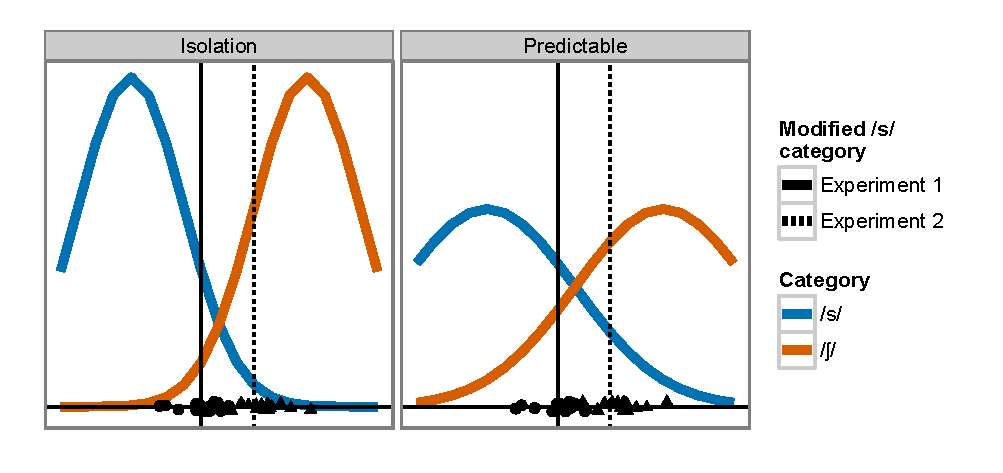
\includegraphics[width=\textwidth]{graphs/distPred}
\end{center}
\end{figure*}

However, if semantic predictability functions in a similar way as consonant cluster coarticulation, listeners would not show perceptual learning effects even if they were tested on a continuum in a high predictability sentence.
In \citet{Kraljic2008a}, listeners exposed to an ambiguous /s/ in the context of /st\textturnr/ and then tested on a continuum from /ast\textturnr i/ to /a\textesh t\textturnr i/ showed no perceptual learning effects.
Participants who were exposed to ambiguous /s/ intervocalically showed perceptual learning on both /asi/-/a\textesh i/ and /ast\textturnr i/-/a\textesh t\textturnr i/ continua.
There was no exposure-specificity effect, so participants did not even learn that the speaker produces a more /\textesh/-like /s/ in that context.
Any abstract encoding process accounts for and removes the variability associated with the context, leaving the unmodified perceptual category.
A similar pattern is likely to be seen with high predictability exposure.
Importantly, the speaker's durations for the target /s/ words did not different across predictability conditions (Predictable /s/ words: mean = 0.53 s, SD = 0.06 s; Unpredictable /s/ words: mean = 0.53 s, SD = 0.07 s).
Any effect of predictability is more likely from listener perception than speaker production in this experiment.

One question raised by this finding is whether perceptual learning is possible at all in high predictability sentences.
If the range of acceptable variation for all categories is expanded (schematized in Figure~\ref{fig:distPred}), the modified category would have fallen closer to the expected mean in predictable sentences compared to isolation.
In terms of error propagation, the modified categories used here may not have generated enough errors to learn from.
Presenting listeners with a more atypical category should then cause more perceptual learning in this case.
In Figure~\ref{fig:distPred}, the atypical category from Experiment 2 would have a higher likelihood of being categorized as /s/ in predictable sentences than in isolation.
If increasing the atypicality in predictable sentences did in fact result in increased perceptual learning, it would suggest that perceptual learning is maximized in a particular range.
Tokens too close to the expected mean are too typical to learn from, and tokens too far from the expected mean are too unreliable.
However, if listeners simply ignore atypical sounds in highly predictable words, then increasing the atypicality of the category (i.e. using the ambiguity threshold from Experiment 2) would not increase perceptual learning.
If that were the case, listeners might not even be sensitive to replacing the /s/ with another sound category entirely (i.e. /f/) in a comprehension-oriented task \citep[but see][]{Samuel1981}.


\begin{figure*}[!ht]
\centering
\caption{Distribution of cross-over points for each participant across comparable exposure tokens in Experiments 1 and 3.  Larger bulges represent more subjects located at that point in the distribution.  The dashed line represents the mean step of the continua.  Large bulges around the dashed line for Control, Unpredictive and Predictive conditions indicate that many speakers did not change their category boundaries, compared to the Isolation conditions.}
\label{fig:exp13xoverdist}
\begin{center}
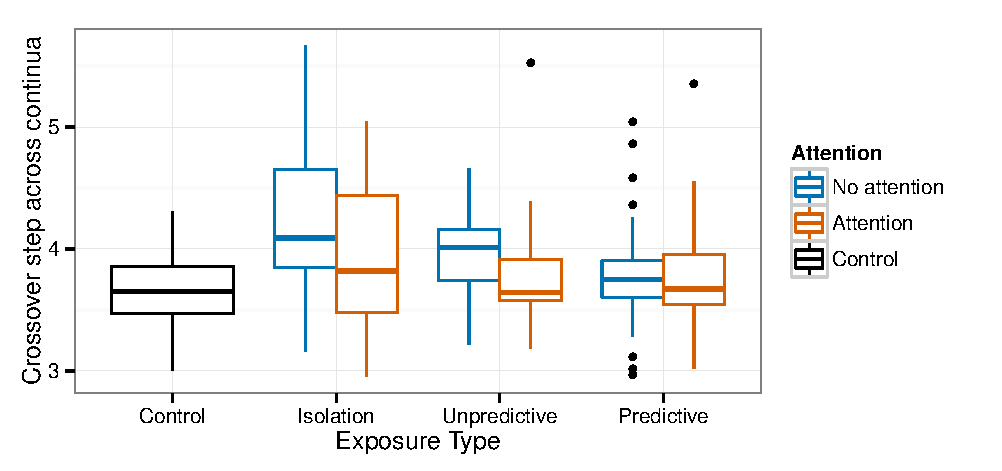
\includegraphics[width=\textwidth]{graphs/exp13_xoverdist}
\end{center}
\end{figure*}

As a final point in this discussion, the distribution of individuals' perceptual learning effects differs in shape as compared to Experiment 1. 
Figure~\ref{fig:exp13xoverdist} shows the distribution of cross-over points of each subject in Experiment 3 and participants in the condition of Experiment 1 that used the same exposure words.  
Cross-over points are where along the continua perception switches from primarily /s/ to primarily /\textesh/, and higher cross-over points are indicative of greater perceptual learning.
Participants exposed to the modified category in sentences show more consistency (larger bulges in the violin plots) than those exposed in isolated words.
In the Isolation conditions, participants follow a fairly wide, even distribution.
In contrast, participants in the sentence conditions a more tightly clustered either around the normalized cross over point or a step above, suggesting potentially discrete groups in the distribution.

One possible reason for these more discrete groups may relate to cognitive load.
Under lower cognitive load conditions, participants in perception-oriented tasks show greater perceptual sensitivity.
In this experiment, the task is comprehension-oriented, so lower cognitive load could have distributed cognitive resources either to the comprehension task or to aspects of the signal.
Participants with better attention-switching control might devote those resources to perception, while those with worse attention-switching control might not, which may be the cause of the findings in \citet{Scharenborg2013}.
Future research should quantify participants' attention-switching abilities and other individual differences that may play a role in explaining these findings.



